\documentclass[11pt]{article}
\usepackage{fullpage,fourier,amsmath,amssymb}
\usepackage{listings,color,url,hyperref}
\usepackage{epigraph, graphicx}
\usepackage[x11names]{xcolor}
\usepackage{tikz}
\usepackage{blkarray}
\usepackage{tcolorbox}
\usepackage[linguistics]{forest}

\title{Assignment 3 \\ Brunch with the Minotaur}
\author{Prof. Darrell Long \\
CSE 13S -- Winter 2020}
\date{Due: February 2$^\text{nd}$ at 11:59\,pm}

\usepackage{fancyhdr}
\pagestyle{fancy}
\fancyhf{}

\fancypagestyle{plain}{%
  \fancyhf{}
  \renewcommand{\headrulewidth}{0pt}
  \renewcommand{\footrulewidth}{0pt}
  \lfoot{\textcopyright{} 2021 Darrell Long}
  \rfoot{\thepage}
}

\pagestyle{plain}

\definecolor{codegreen}{rgb}{0,0.5,0}
\definecolor{codegray}{rgb}{0.5,0.5,0.5}
\definecolor{codepurple}{rgb}{0.58,0,0.82}

\lstloadlanguages{C,make,python,fortran}

\lstdefinestyle{c99}{
    morekeywords={bool, uint8_t, uint16_t, uint32_t, uint64_t, int8_t, int16_t, int32_t, int64_t},
    commentstyle=\color{codegreen},
    keywordstyle=\color{magenta},
    numberstyle=\tiny\color{codegray},
    identifierstyle=\color{blue},
    stringstyle=\color{codepurple},
    basicstyle=\ttfamily,
    breakatwhitespace=false,
    breaklines=true,
    captionpos=b,
    keepspaces=true,
    numbers=left,
    numbersep=5pt,
    showspaces=false,
    showstringspaces=false,
    showtabs=false,
    tabsize=4
}

\lstset{language=C, style=c99}
\newtcolorbox{prelab}[1]{colback=red!5!white, colframe=red!75!black, title=#1}
\newcommand\asgn[1]{asgn#1}


\begin{document}\maketitle

%%%%%%%%%%%%%%%%%%%%%%%%%%%%%%%%%%%%%%%%%%%%%%%%%%%%%%%%

\section{Introduction}

\epigraphwidth=0.65\textwidth \epigraph{\emph{``How beautiful the world is, and
how ugly labyrinths are,'' I said, relieved. ``How beautiful the world would be
if there were a procedure for moving through labyrinths,'' my master
replied.}}{---Umberto Eco, \emph{The Name of the Rose}}

\noindent You and your comrades are hanging out at Coachella, and come across a
man named Aegeus.  Seeing that he is a charming and likeable man, you and your
comrades decide that it is probably fine to get to know him a bit more. As the
night progresses, you learn more and more interesting tidbits of information
regarding his background.  You learn that he is from Greece, and is incredibly
tight with two blokes, Minos and Daedalus.  Aegeus takes a liking to your band
of friends and invites you to an island off the coast of Crete. Very
suspicious.  You and your comrades politely decline and turn in for the night,
only to awake and find yourselves no longer at Coachella, but instead trapped
within a ring of entrances to a labyrinth; labyrinthine paths as far as the eye
can see. Suddenly it hits you.  \emph{Minos} is the name of the first king of
Crete, who asked King \emph{Aegeus} to send fourteen young children annually
into \emph{Daedalus}' labyrinth, the abode of the fearsome Minotaur. Your
skills as an aspiring computer scientist are now put to work. You set out to
code up a program that, when fed the blueprints of a labyrinth, will print out
all possible paths through the labyrinth, the number of paths, and the length of
the shortest path.  In order to code this up however, you realize you must
decide how to represent a labyrinth, how to traverse a labyrinth, and finally,
how to keep track of the paths taken through a labyrinth.

\section{Representing the Labyrinth}
\epigraphwidth=0.75\textwidth
\epigraph{\emph{ ``Or like that other Templar, Freud,'' Belbo said, ``who
instead of probing the labyrinths of the physical underground, probed those of
the psychic underground, as if everything about them hadn't already been said,
and better, by the alchemists.''}}{---Umberto Eco, \emph{Foucault's Pendulum}}

\noindent You remember that there is a data structure called a \emph{graph}. A
graph is comprised of a set of points (called \emph{vertices}) and a set of
lines (called \emph{edges}) that connect pairs of distinct vertices. Two
vertices that are connected with an edge are \emph{adjacent} to one another.
Each junction in a labyrinth will be a vertex in a graph, and the hallways
connecting junctions are edges. There are two types of edges: \emph{undirected}
and \emph{directed}. A directed edge is much like a one-way street, in that you
can only go from the starting vertex and end at the ending vertex. An undirected
edge can be thought of as two one-way streets running in parallel and in
opposite directions, or as just a two-way street.

\begin{center}
    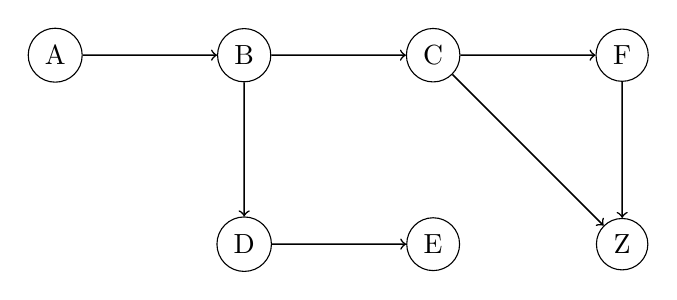
\begin{tikzpicture}
  [scale=.8,auto=left,every node/.style={circle,draw=black}]
  \node (A) at (1,10)   {A};
  \node (B) at (4,10)   {B};
  \node (C) at (7,10)   {C};
  \node (D) at (4,7)    {D};
  \node (E) at (7,7)    {E};
  \node (F) at (10,10)  {F};
  \node (Z) at (10,7)   {Z};

  \foreach \from/\to in {A/B,B/C,B/D,D/E,C/F,C/Z,F/Z}
  \draw [line width=0.2mm,->] (\from) -- (\to);

\end{tikzpicture}
\end{center}

For simplicity, you decide to limit your labyrinth to have at most 26 junctions,
meaning the corresponding graph will have at most 26 vertices. Each vertex will
have its own index $i$ such that $0 \leq i \leq 25$. The vertices will have a
one-to-one correspondence with the uppercase characters of the English
alphabet. This means that index 0 corresponds to $\mathbb{A}$, index 1 corresponds to
$\mathbb{B}$, and so on and so forth. By using these indices, you can then represent
edges between vertices in the graph using an \emph{adjacency matrix}. In an
adjacency matrix, a directed edge starting from vertex $i$ and ending at vertex
$j$ exists if \text{matrix}[i][j] = 1. From the graph above, we can see the
following edges: $\mathbb{A}$ to $\mathbb{B}$, $\mathbb{B}$ to $\mathbb{C}$, $\mathbb{B}$ to
$\mathbb{D}$,
$\mathbb{C}$ to $\mathbb{F}$, $\mathbb{C}$ to $\mathbb{Z}$, to $\mathbb{D}$ to $\mathbb{E}$.
These edges are represented using the following adjacency matrix:

\begin{center}
\begin{blockarray}{ccccccccc}
 & A & B & C & D & E & F & $\dotsi$ & Z\\
\begin{block}{c[>{\medspace}cccccccc<{\medspace}]}
    A & 0 & 1 & 0 & 0 & 0 & 0 & 0 & 0 \\
    B & 0 & 0 & 1 & 1 & 0 & 0 & 0 & 0 \\
    C & 0 & 0 & 0 & 0 & 0 & 1 & 0 & 1 \\
    D & 0 & 0 & 0 & 0 & 1 & 0 & 0 & 0 \\
    E & 0 & 0 & 0 & 0 & 0 & 0 & 0 & 0 \\
    F & 0 & 0 & 0 & 0 & 0 & 0 & 0 & 0 \\
    \smash{\vdots} & 0 & 0 & 0 & 0 & 0 & 0 & 0 & 0 \\
    Z & 0 & 0 & 0 & 0 & 0 & 0 & 0 & 0 \\
\end{block}
\end{blockarray}
\end{center}

The input to your program will be a file containing pairs of characters
separated by a newline. The example below shows the contents of the file that
would be supplied to your program to generate the adjacency matrix above.

\begin{lstlisting}[title=Example input of graph edges.]
    AB
    BC
    BD
    CF
    CZ
    DE
\end{lstlisting}

We have chosen to represent an undirected graph as a pair of edges
$x\rightarrow y$ and $y\rightarrow x$. That means that every
undirected edge really has two entries in the adjacency matrix,
rather like a two way road having a lane going in each direction.
If the edges were really undirected, where $x\leftrightarrow y$,
then we only would have $\text{matrix}[x][y] = 1$ and that would yield an upper-diagonal
matrix. This would be like a road with no lanes (but without any
increased probability of head-on collisions).  It's merely a question
of how we represent the graph, and we have chosen directed edges
since it allows us to have both kinds of graph using the same matrix.

Note that the above examples showcase a \emph{directed} graph. Let's see
what the adjacency matrix and corresponding graph look like when we make each
connection undirected. We know that if $\text{matrix}[i][j] = 1$, then it means
that there is a connection starting from $i$ and ending at $j$. Thus, to make
things undirected, we simply have to set $\text{matrix}[j][i] = 1$. Using the
same input as before, the resulting adjacency matrix would be:

\begin{center}
\begin{blockarray}{ccccccccc}
 & A & B & C & D & E & F & $\dotsi$ & Z\\
\begin{block}{c[>{\medspace}cccccccc<{\medspace}]}
    A & 0 & 1 & 0 & 0 & 0 & 0 & 0 & 0 \\
    B & 1 & 0 & 1 & 1 & 0 & 0 & 0 & 0 \\
    C & 0 & 1 & 0 & 0 & 0 & 1 & 0 & 1 \\
    D & 0 & 1 & 0 & 0 & 1 & 0 & 0 & 0 \\
    E & 0 & 0 & 0 & 1 & 0 & 0 & 0 & 0 \\
    F & 0 & 0 & 1 & 0 & 0 & 0 & 0 & 0 \\
    \smash{\vdots} & 0 & 0 & 0 & 0 & 0 & 0 & 0 & 0 \\
    Z & 0 & 0 & 1 & 0 & 0 & 0 & 0 & 0 \\
\end{block}
\end{blockarray}
\end{center}

We can see that the adjacency matrix for the undirected graph is
the same as the adjacency matrix for the directed graph, but \emph{reflected
across the diagonal}, yielding a symmetric square matrix. The undirected graph
would then be:

\begin{center}
    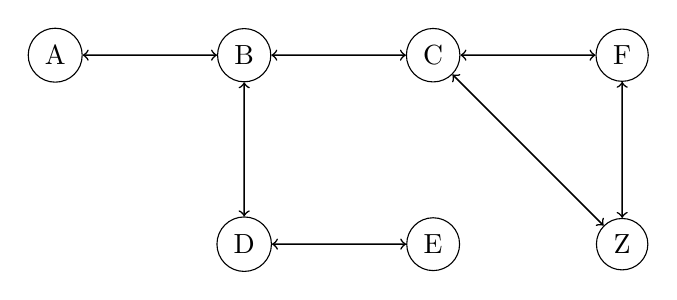
\begin{tikzpicture}
  [scale=.8,auto=left,every node/.style={circle,draw=black}]
  \node (A) at (1,10)   {A};
  \node (B) at (4,10)   {B};
  \node (C) at (7,10)   {C};
  \node (D) at (4,7)    {D};
  \node (E) at (7,7)    {E};
  \node (F) at (10,10)  {F};
  \node (Z) at (10,7)   {Z};

  \foreach \from/\to in {A/B,B/C,B/D,D/E,C/F,C/Z,F/Z}
  \draw [line width=0.2mm,<->] (\from) -- (\to);

\end{tikzpicture}
\end{center}

\begin{figure}[ht]
\centering
{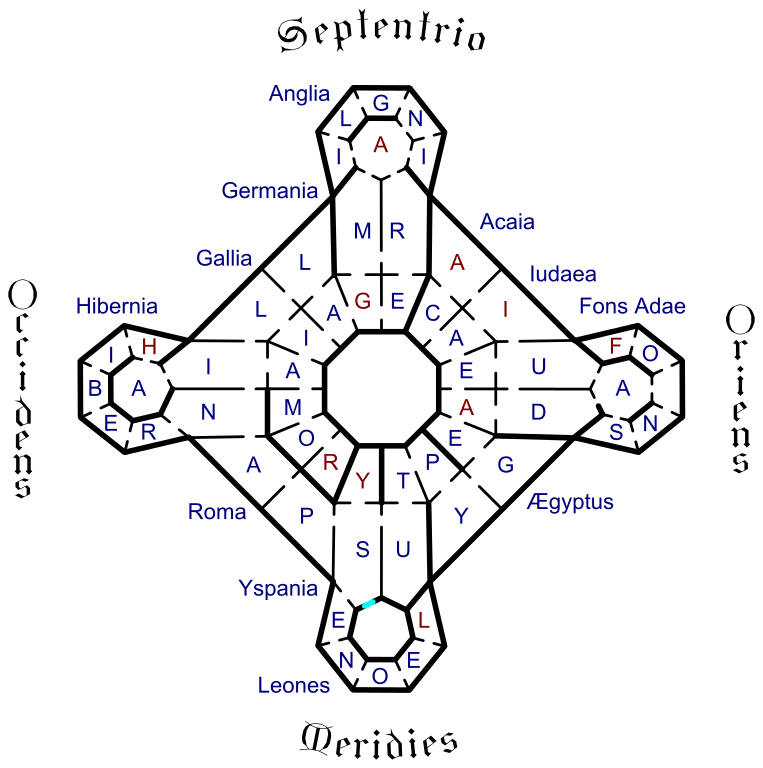
\includegraphics[width=0.5\textwidth]{Labyrinthus.png}} 
\medskip \\
{\emph{Secretum
finis Africae manus supra idolum age primum et septimum de quatuor.}}
\end{figure}

\section{Traversing the Labyrinth}

\epigraphwidth=0.85\textwidth \epigraph{\emph{``To find the way out of a
        labyrinth,'' William recited, ``there is only one means. At every new
        junction, never seen before, the path we have taken will be marked with
        three signs. If, because of previous signs on some of the paths of the
junction, you see that the junction has already been visited, you will make only
one mark on the path you have taken. If all the apertures have already been
marked, then you must retrace your steps \ldots''}}{---Umberto Eco, \emph{The
Name of the Rose}}

\noindent You decide to use a simple recursive backtracking algorithm to
traverse through the labyrinth. Recursive backtracking is an algorithm that is used to build a solution incrementally, one step at a time, by removing those solutions which fail to satisfy the constraints of the problem at any given condition or time. The idea behind backtracking to find paths through a labyrinth is quite straightforward: starting from the entrance of a labyrinth, try going down hallway connected to each junction you come
across. If a dead-end is reached after going down a hallway, simply backtrack to
the previous junction you were in and try a different hallway. In the event that
you find the exit of the labyrinth, record the current path taken and backtrack
to try to find other paths. \emph{Important:} a path through a labyrinth in our example
means that, starting from node $\mathbb{A}$, it is possible to reach node $\mathbb{Z}$. \\

An example of a backtracking traversal algorithm is \emph{Depth
First Search (DFS)}. For the most recently discovered vertex \textit{v},
which still has unexplored edges, DFS explores edges out of \textit{v}
(not including \textit{v}). Once the algorithm has explored all
edges of \textit{v}, it backtracks to explore other edges leaving
the vertex from which \textit{v} was originally discovered. In case
of undiscovered vertices, DFS selects a new source vertex and repeats
the search from the source. This process continues until every
vertex has been explored.

\begin{center}
    \begin{forest}
  [$1$[$2$[$4$][$5$]][$3$]]
\end{forest}
\end{center}

An example of DFS is post order traversal, where the algorithm first looks at a the left node, followed by the right node and then finally the root node. In the case of the tree provided above, the post order DFS traversal would search the nodes in the order $(4, 5, 2, 3, 1)$.  

\begin{prelab}{Pre-lab Part 1}
    \begin{enumerate}
        \item Write pseudocode for creating the adjacency matrix from a file
            with contents similar to the example input file.
        \item Given the graph above, draw and list the recursive traversal of
            the graph.  This can be done by naming each edge by it's adjacent
            nodes where edge \textit{AB} is the edge from \textit{A} to
            \textit{B} and listing the order in which the edges are taken.
        \item Looking at the post order traversal for the tree above, find the worse case complexity of the traversal algorithm. 
    \end{enumerate}
\end{prelab}

\section{Tracking the Paths}
\epigraphwidth=0.9\textwidth \epigraph{\emph{ Zu Mittag theilte Grethel ihr Brot
        mit H\"ansel, weil der seins all auf den Weg gestreut hatte, aber der
        Mittag verging und der Abend verging, und niemand kam zu den armen
        Kindern. H\"ansel tr\"ostete die Grethel und sagte: ``wart, wenn der
        Mond aufgeht, dann seh ich die Br\"ocklein Brot, die ich ausgestreut
        habe, die zeigen uns den Weg nach Haus.'' Der Mond ging auf, wie aber
        H\"ansel nach den Br\"ocklein sah, da waren sie weg, die viel tausend
        V\"oglein in dem Wald, die hatten sie gefunden und
aufgepickt.}}{---Br\"uder Grimm}

% \epigraphwidth=0.75\textwidth \epigraph{\emph{The worst labyrinth is not that
% intricate form that can entrap us forever, but a single and precise straight
% line.}}{---Jorge Luis Borges}

\noindent
You're keenly aware that your program must keep track of the current path while
traversing a labyrinth, but how best to do so? The brilliant idea of using a
\emph{stack} comes to you.

A stack is a linear data structure that follows either a LIFO
(last-in, first-out) or FILO (first-in, last-out) order. The two main stack
operations pushing and popping. A good example of a stack would be a stack of
plates in a cupboard. Pushing a plate into this stack would mean placing the
plate on the very top. Popping a plate off this stack would mean removing the
plate on the very top.

The stack will be utilized in the following fashion: whenever a new junction is
reached, the new junction is pushed into the stack. Whenever a dead-end is
reached, we pop the current junction from the stack and backtrack. Whenever the
exit of a labyrinth has been reached, the stack is printed to display a valid
path through the labyrinth. Again, a path through a labyrinth means that it is
possible to go from node $\mathbb{A}$ to node $\mathbb{Z}$.

Below is the header file for the stack abstract data type (ADT) that you are
required to implement for this assignment.  Note that there is only a
\texttt{stack\_empty()} function, and not a \texttt{stack\_full()} function.
This is because you will be implementing a dynamic stack; the capacity is
doubled whenever the current stack capacity has been reached, meaning the stack
can never be full. You can find a example of a dynamic stack in the lecture
slides, but be sure to cite it if you decide to use it.

\begin{lstlisting}[title=stack.h]
#ifndef __STACK_H__
#define __STACK_H__

#include <inttypes.h>
#include <stdbool.h>

#define MINIMUM 26

typedef struct Stack {
  uint32_t *items;      // A stack holds uint32_t.
  uint32_t top;         // Keeps track of the top index of a stack.
  uint32_t capacity;    // Keeps track of a stack's capacity.
} Stack;

Stack *stack_create(void);

//
// Constructor for a stack.
// A stack is initialized to hold MINIMUM number of uint32_t.
//
// returns: A pointer to the constructed stack.
//

void stack_delete(Stack *s);

//
// Destructor for a stack.
//
// returns: Void.
//

bool stack_empty(Stack *s);

//
// Checks if a stack is empty.
//
// returns: True is the stack is empty, false otherwise.
//

uint32_t stack_size(Stack *s);

//
// returns: The number of items currently in the stack.
//

bool stack_push(Stack *s, uint32_t item);

//
// Pushes an item (a uint32_t) into the stack.
//
// returns: True if the item was pushed, false otherwise.
//

bool stack_pop(Stack *s, uint32_t *item);

//
// Pops an item (a uint32_t) off the stack.
// The value of the popped item is stored in the supplied pointer.
// Ex.: *item = popped_value
//
// returns: True if the item was popped, false otherwise.
//

void stack_print(Stack *s);

//
// Function that prints out the contents of a stack.
// Refer to program output for print format.
//
// returns: Void.
//


#endif
\end{lstlisting}

\begin{prelab}{Pre-lab Part 2}
    \begin{enumerate}
        \item Provide pseudocode for each stack ADT function shown above.
    \end{enumerate}
\end{prelab}

\section{Specifics}
\epigraphwidth=0.65\textwidth \epigraph{\emph{There is no idea so stupid that
you can't find a professor who will believe it.}} {---H. L. Mencken}

Your executable program must be named \texttt{pathfinder} and must support the
following \texttt{getopt()} arguments:

\begin{enumerate}
    \item \texttt{-i <input>} : specifies \texttt{<input>} as the file
        containing the edges of a graph (default input should be
        \texttt{stdin}).
    \item \texttt{-u} : specifies that the graph be undirected (this is the
        default).
    \item \texttt{-d} : specifies that the graph be directed.
    \item \texttt{-m} : specifies that the adjacency matrix be printed.
\end{enumerate}

You must be able to support any combination of these flags, except for the
``\texttt{-u}'' and ``\texttt{-d}'' flags, which if both are specified should result in an error.
Again, \emph{undirected edges} should be the default of your program.

There will be some example input files made available to you, as well as
corresponding output files, for you to base your program output off of. Other
specifications:

\begin{itemize}
\item The file that contains the \texttt{main()} function for your program must
    be named \texttt{pathfinder.c}. Do not name it anything else.
    \textcolor{red}{You will lose points}.
\item The executable generated by your \texttt{Makefile} must be named
    \texttt{pathfinder}. It cannot be named anything else. \textcolor{red}{You
    will lose a \emph{lot} of points}.
\item Typing \texttt{make} must build your program. This means no errors and no
    warnings when using the compiler flags supplied in the coding standards and
    in previous assignments.
\item All source code must be formatted \texttt{clang-format}.
\item Your program \emph{must} run on the time share. If it does not, your
    program will receive a 0. To avoid this, test your program on the time
    share.
\item Your program must pass \texttt{infer} with no errors. If there are any,
    fix them; for those that you cannot fix, make sure to document them in your
    \texttt{README}.
\end{itemize}

\section{Hints}
\epigraphwidth=0.65\textwidth
\epigraph{\emph{It is no use trying to sum people up. One must follow hints,
not exactly what is said, nor yet entirely what is done.}}{---Virginia Woolf}

\begin{enumerate}
    \item Start first by implementing your stack ADT. Code up a test harness for
        it and test each stack operation.
    \item Familiarize yourself with opening files in \textbf{C}. You will most
        likely want to use \texttt{fopen()} to open files for reading, and
        \texttt{fscanf()} to read in the pairs from the supplied input file.
        Read the manpage on both for more details.
    \item You will likely want to look into the functions \texttt{isalpha()} and
        \texttt{toupper()} when reading in the pairs and converting them into
        integers between 0 --- 25 inclusive.
    \item Write your recursive function to traverse through a labyrinth. To help
        you get started, here's some pseudocode:
\begin{lstlisting}
Initialize path stack.

void dfs(uint32_t curr_node):
  if curr_node is the exit:
    print current path
    return

  for all possible next_node:
    path.push(curr_node)
    dfs(next_node)
    path.pop()

  return
\end{lstlisting}
    \item Think carefully about traversing the labyrinth. Should you go back
        into a junction you've already visited? How should you keep track of
        which junctions you've visited? An array, perhaps?
\end{enumerate}

\section{Deliverables}
\epigraphwidth=0.65\textwidth
\epigraph{\emph{The design process is about designing and prototyping and
making. When you separate those, I think the final result
suffers.}}{---Jonathan Ive}

You will need to turn in:

\begin{enumerate}
    \item \texttt{pathfinder.c}: The source file containing your program's
        \texttt{main()} function.
    \item \texttt{stack.c} and \texttt{stack.h}: The files containing your
        implemented stack ADT.
    \item \texttt{Makefile}: Allows the grader to type \texttt{make} to build
        your program.
    \begin{itemize}
        \item The compiler flags: \texttt{-Wall -Wextra -Werror -Wpedantic} must
            be included.
        \item The compiler used must be \texttt{clang}.
        \item \texttt{make clean} must remove all compiler generated files.
        \item \texttt{make infer} must build and run \texttt{infer} on your
            program, passing without errors. Again, any errors that you cannot
            fix should be documented in your \texttt{README}.
        \item \texttt{make} should build your program, as should \texttt{make
            all}.
        \item Your program executable must be named \texttt{pathfinder}.
    \end{itemize}
    \item \texttt{README.md}: This must be in markdown.  This must describe how
        to use your program and \texttt{Makefile}.
    \item \texttt{DESIGN.pdf}: This \emph{must} be a PDF. The design document
        should contain answers to the pre-lab questions in the beginning and
	describe your design for your program with enough detail that a
        sufficiently knowledgeable programmer would be able to replicate your
        implementation. This does not mean copying your entire program in
        verbatim. You should instead describe how your program works with
	supporting pseudocode. 

You \emph{must} push the \texttt{DESIGN.pdf} before you
	push \textcolor{red}{\emph{any}} code.
    \item \texttt{WRITEUP.pdf}: This PDF will contain an explanation of your thoughts on the following:
             \begin{enumerate}
                \item Contemplate the number of possible paths that you can take to achieve the expected outcome.
                \item Is this an inherently hard computational problem?
             \end{enumerate}
\end{enumerate}

All of these files must be in the directory \texttt{\asgn{3}}.

\section{Submission}
\epigraphwidth=0.5\textwidth
\epigraph{\emph{Better three
hours too soon than a minute too late.}}{---William Shakespeare}

To submit your assignment, follow the steps on how
to submit your assignment through \texttt{git}. Remember: \emph{add, commit,}
and \emph{push}!

\begin{enumerate}
\item Add it!
\begin{lstlisting}
git add file_name.c
\end{lstlisting}
As mentioned before, you will need to first add the files to
your repository using the \texttt{git add <filenames>} command. You
will be submitting these files into the \texttt{\asgn}
directory.

\item Commit it!
\begin{lstlisting}
git commit -m "Your commit message here"
\end{lstlisting}
Changes to these files will be committed to the repository with
\texttt{git commit}. The command should also include a commit message
describing what changes are included in the commit. For your final and last commit for submission, your commit message should be ``final submission''.

\item Push it!
\begin{lstlisting}
git push
\end{lstlisting}
The committed changes are then synch'd up with the remote server
using the \texttt{git push} command. You must be sure to push your
changes to the remote server or else they will not be received by
the graders.

\end{enumerate}

\textcolor{red}{Your assignment is turned in \emph{only} after you have pushed.
If you forget to push, you have not turned in your assignment and you will get a
\emph{zero}. ``I forgot to push'' is not a valid excuse. It is \emph{highly}
recommended to commit and push your changes \emph{often}.}

%%%%%%%%%%%%%%%%%%%%%%%%%%%%%%%%%%%%%%%%%%%%%%%%%%%%%%%%

\centerline{
\includegraphics[width=0.5\textwidth]{../assignment1/obey.jpg}}




\section{Supplemental Readings}
\epigraph{\emph{The more you read, the more things you will know. The
more that you learn, the more places you'll go.}}{---Dr.\ Seuss}\noindent

\begin{itemize}
    \item \textit{The C Programming Language} by Kernighan \& Ritchie
    \begin{itemize}
        \item Chapter 4 \S 4.5--4.11
	\item Chapter 5 \S 5.1--5.5, 5.7
	\item Chapter 6 \S 6.1--6.2, 6.7
    \end{itemize}

    \item \textit{The Art of Computer Programming} by Donald E.Knuth
    \begin{itemize}
        \item Chapter 2 \S 2.3.4.1
    \end{itemize}

    \item \textit{Wikipedia}
    \begin{itemize}
	\item \href{https://en.wikipedia.org/wiki/Graph_theory}{Graph Theory}
	\item \href{https://en.wikipedia.org/wiki/Depth-first_search}{DFS}
    \end{itemize}
\end{itemize}

\begin{figure}[ht]
  \centering
    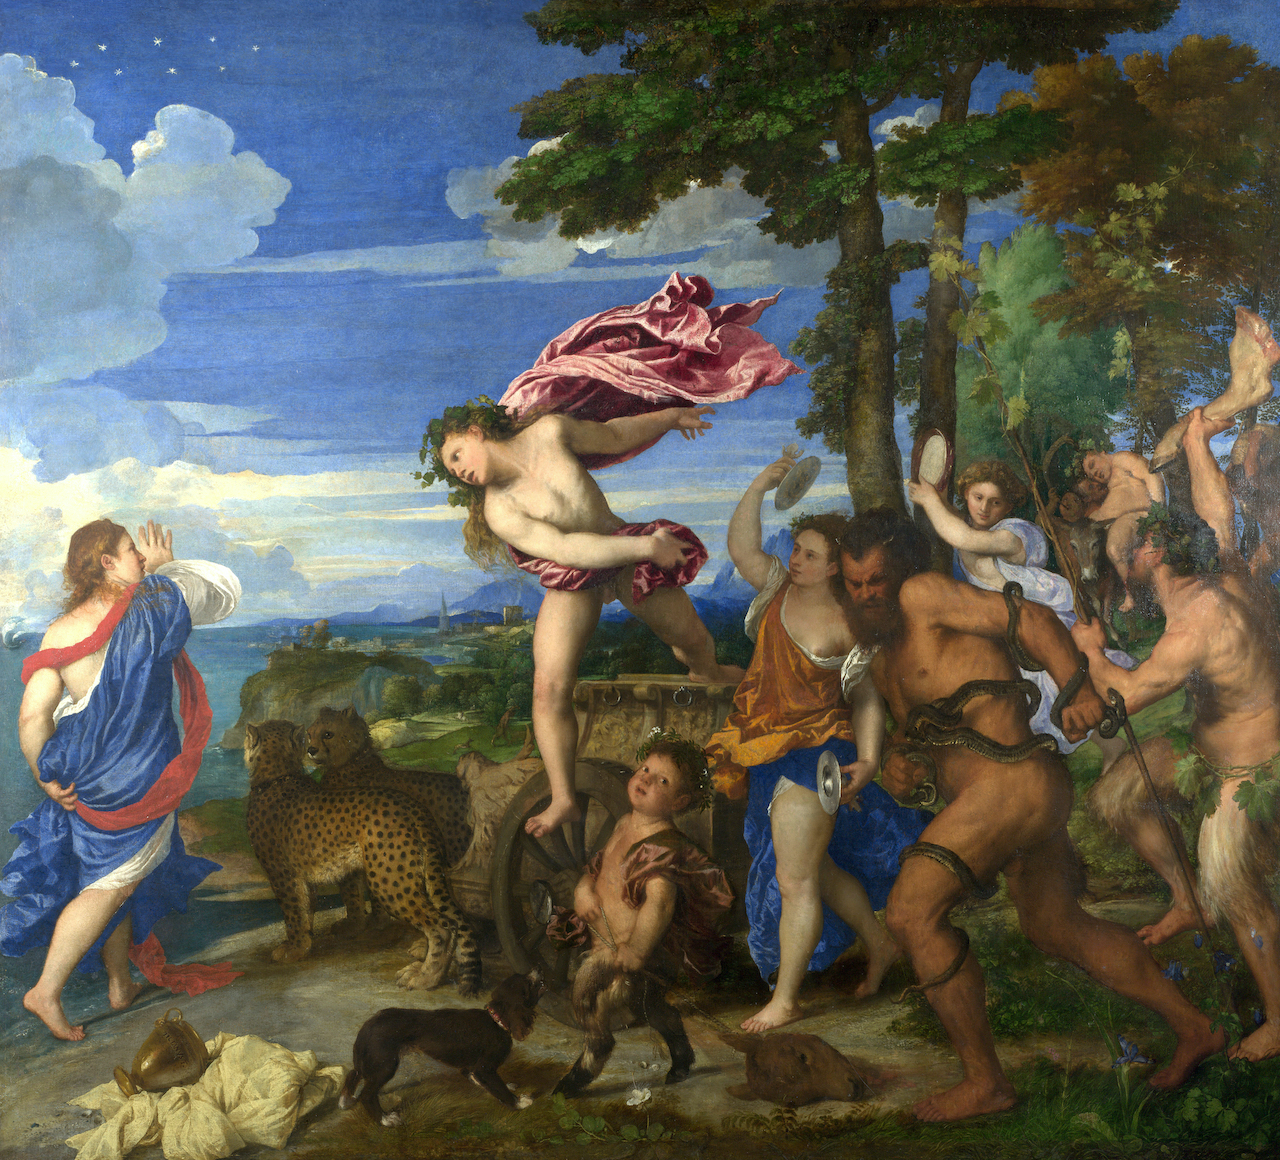
\includegraphics[width=0.9\textwidth]{Titian_Bacchus_and_Ariadne.jpg}
\medskip \\
{Partying with Ariadne---What could possibly go wrong?}\label{bacchus}
\end{figure}

\end{document}
